\section{Abstract}
This project used Kepler's laws to generate the orbits of Earth and Mars, and to map the distance between the two
planets over time. The distance between the two at a given time was approximated by assigning constant velocities to
small fractions of the planets' orbits. The final result of the distance function was innacurate, likely due to the 
method of approximation, but the exact reason is unclear.
\section{Introduction}
This project uses an integration approximation method to generate the positions of Earth and Mars at a given time. 
The final result is not expected to be fully accurate as the tilt of Mars' orbit relative to the Earth's was not 
considered. Nevertheless, the purpose of this project was to experiment with an approximation method of modeling and
comparing the orbits of two planets. Since all the planetary data is loaded in from a text file, modeling planets other than Earth and Mars is as simple as changing the start positions, semimajor axes, and eccentricities contained in the 
text file. 
The relevent equations were taken from Classical Mechanics by Taylor \cite{taylor_classical_2005} and the Website "HyperPhysics by "Georgia State University
\cite{noauthor_Keplers_nodate}. The Georgia State
website was also the source of the eccentricities and semi-major axes. 
The starting positions for Earth and Mars were approximated using the application Solar System Scope, based on March 31,2021\cite{noauthor_solar_nodate}.
This was a rough estimate, but the application was the best that could be found. The other relevent constants (mass of
the sun and the gravitational constant "G" were considered common knowledge).
Figure (\ref{OrbitPlot}) was created
based on Kepler's laws found in Classical Mechanics by Taylor, and relevant constants.
\begin{figure}
	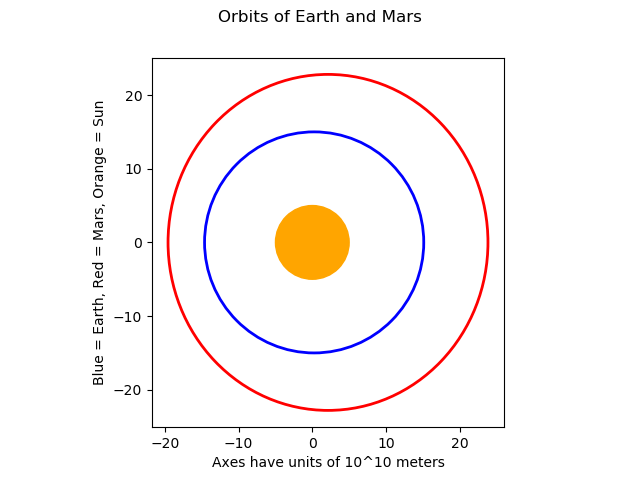
\includegraphics[scale = 0.8]{EllipseTest2.png}
	\label{OrbitPlot}
	\caption{Orbits of Earth and Mars based on Kepler's laws. Orbital tilt is not considered}
\end{figure}
